\documentclass[twoside]{book}

% Packages required by doxygen
\usepackage{fixltx2e}
\usepackage{calc}
\usepackage{doxygen}
\usepackage[export]{adjustbox} % also loads graphicx
\usepackage{graphicx}
\usepackage[utf8]{inputenc}
\usepackage{makeidx}
\usepackage{multicol}
\usepackage{multirow}
\PassOptionsToPackage{warn}{textcomp}
\usepackage{textcomp}
\usepackage[nointegrals]{wasysym}
\usepackage[table]{xcolor}

% NLS support packages
\usepackage[brazil]{babel}
% Font selection
\usepackage[T1]{fontenc}
\usepackage[scaled=.90]{helvet}
\usepackage{courier}
\usepackage{amssymb}
\usepackage{sectsty}
\renewcommand{\familydefault}{\sfdefault}
\allsectionsfont{%
  \fontseries{bc}\selectfont%
  \color{darkgray}%
}
\renewcommand{\DoxyLabelFont}{%
  \fontseries{bc}\selectfont%
  \color{darkgray}%
}
\newcommand{\+}{\discretionary{\mbox{\scriptsize$\hookleftarrow$}}{}{}}

% Page & text layout
\usepackage{geometry}
\geometry{%
  a4paper,%
  top=2.5cm,%
  bottom=2.5cm,%
  left=2.5cm,%
  right=2.5cm%
}
\tolerance=750
\hfuzz=15pt
\hbadness=750
\setlength{\emergencystretch}{15pt}
\setlength{\parindent}{0cm}
\setlength{\parskip}{3ex plus 2ex minus 2ex}
\makeatletter
\renewcommand{\paragraph}{%
  \@startsection{paragraph}{4}{0ex}{-1.0ex}{1.0ex}{%
    \normalfont\normalsize\bfseries\SS@parafont%
  }%
}
\renewcommand{\subparagraph}{%
  \@startsection{subparagraph}{5}{0ex}{-1.0ex}{1.0ex}{%
    \normalfont\normalsize\bfseries\SS@subparafont%
  }%
}
\makeatother

% Headers & footers
\usepackage{fancyhdr}
\pagestyle{fancyplain}
\fancyhead[LE]{\fancyplain{}{\bfseries\thepage}}
\fancyhead[CE]{\fancyplain{}{}}
\fancyhead[RE]{\fancyplain{}{\bfseries\leftmark}}
\fancyhead[LO]{\fancyplain{}{\bfseries\rightmark}}
\fancyhead[CO]{\fancyplain{}{}}
\fancyhead[RO]{\fancyplain{}{\bfseries\thepage}}
\fancyfoot[LE]{\fancyplain{}{}}
\fancyfoot[CE]{\fancyplain{}{}}
\fancyfoot[RE]{\fancyplain{}{\bfseries\scriptsize Gerado por Doxygen }}
\fancyfoot[LO]{\fancyplain{}{\bfseries\scriptsize Gerado por Doxygen }}
\fancyfoot[CO]{\fancyplain{}{}}
\fancyfoot[RO]{\fancyplain{}{}}
\renewcommand{\footrulewidth}{0.4pt}
\renewcommand{\chaptermark}[1]{%
  \markboth{#1}{}%
}
\renewcommand{\sectionmark}[1]{%
  \markright{\thesection\ #1}%
}

% Indices & bibliography
\usepackage{natbib}
\usepackage[titles]{tocloft}
\setcounter{tocdepth}{3}
\setcounter{secnumdepth}{5}
\makeindex

% Hyperlinks (required, but should be loaded last)
\usepackage{ifpdf}
\ifpdf
  \usepackage[pdftex,pagebackref=true]{hyperref}
\else
  \usepackage[ps2pdf,pagebackref=true]{hyperref}
\fi
\hypersetup{%
  colorlinks=true,%
  linkcolor=blue,%
  citecolor=blue,%
  unicode%
}

% Custom commands
\newcommand{\clearemptydoublepage}{%
  \newpage{\pagestyle{empty}\cleardoublepage}%
}

\usepackage{caption}
\captionsetup{labelsep=space,justification=centering,font={bf},singlelinecheck=off,skip=4pt,position=top}

%===== C O N T E N T S =====

\begin{document}

% Titlepage & ToC
\hypersetup{pageanchor=false,
             bookmarksnumbered=true,
             pdfencoding=unicode
            }
\pagenumbering{alph}
\begin{titlepage}
\vspace*{7cm}
\begin{center}%
{\Large Programa de Venda \\[1ex]\large 1.\+0 }\\
\vspace*{1cm}
{\large Gerado por Doxygen 1.8.13}\\
\end{center}
\end{titlepage}
\clearemptydoublepage
\pagenumbering{roman}
\tableofcontents
\clearemptydoublepage
\pagenumbering{arabic}
\hypersetup{pageanchor=true}

%--- Begin generated contents ---
\chapter{L\+E\+IA ME -\/ Programa de Venda v1.0}
\label{index}\hypertarget{index}{}O \hyperlink{class_programa}{Programa} de Venda é um {\itshape software} para organização de vendas, clientes e estoque de produtos em um comércio.

\subsection*{Dependências}

Bibliotecas de C++ necessárias\+:


\begin{DoxyCode}
<climits>
<fstream>
<functional>
<iomanip>
<iostream>
<map>
<string>
<vector>
\end{DoxyCode}


\subsection*{Instalação}

No terminal digite o seguinte comando\+:


\begin{DoxyCode}
make
\end{DoxyCode}


E depois digite o outro comando\+:


\begin{DoxyCode}
make run
\end{DoxyCode}


Se for feita alguma alteração nos arquivos, é necessário entrar com o seguinte comando antes dos outros anteriores\+:


\begin{DoxyCode}
make clean
\end{DoxyCode}


\subsection*{Utilização}

\subsubsection*{Menu}

\begin{DoxyVerb}    ***************************************************
    *     Bem vindo ao seu Programa de Venda v1.0     *
    *             (c) 1991 - Ítalo Alves              *
    ***************************************************

    Para entrar no Modo Venda digite 1
    Para entrar no Modo Estoque digite 2
    Para entrar no Modo Recomendação digite 3
    Para mais informações abra o arquivo LEIAME.
\end{DoxyVerb}



\begin{DoxyItemize}
\item A tela inicial do programa é o {\bfseries Menu}, nele você pode entrar em qualquer Modo\+: basta digitar o número correspondente e teclar {\itshape Enter}.
\item Para todas as opções em qualquer Modo se digita o número e pressiona a tecla {\itshape Enter}. 


\end{DoxyItemize}

\subsubsection*{1. Modo Venda}

\begin{DoxyVerb}[Modo Venda]

    Produtos em estoque:

    Produto 1                     Valor: $10.00               Estoque: 5                   ID: 1
    Produto 2                     Valor: $5.00                Estoque: 2                   ID: 2
    Produto 3                     Valor: $1.99                Estoque: 10                  ID: 3

Adicione produtos ao carrinho inserindo o código (ID)
Digite somente 0 para ir ao carrinho.
\end{DoxyVerb}



\begin{DoxyItemize}
\item Ao entrar no {\bfseries Modo Venda}, é exibido os produtos em estoque que estão prontos para a compra.
\item Para adicionar o produto ao carrinho, digite o ID correspondente e tecle {\itshape Enter}.
\item Digite 0 no lugar de ID do produto para ir ao carrinho. ~\newline

\end{DoxyItemize}

\begin{DoxyVerb}    Insira o código do produto: 1
    Item 'Produto 1' adicionado.

    Insira o código do produto: 2
    Item 'Produto 2' adicionado.

    Insira o código do produto: 2
    Item 'Produto 2' acrescentado.

    Insira o código do produto: 0
\end{DoxyVerb}



\begin{DoxyItemize}
\item Após adicionar os produtos desejados e ter digitado 0, o carrinho é mostrado. ~\newline

\end{DoxyItemize}

\begin{DoxyVerb}    Produtos no carrinho (2):

    Produto 1                     Valor: $10.00               Quantidade: 1                   ID: 1
    Produto 2                     Valor: $5.00                Quantidade: 2                   ID: 2                   

    Total: $15.00               Valor dos produtos: $15.00               Desconto: $0.00                

Para seguir com o checkout digite 0
Para voltar e continuar adicionando produtos, digite 1
Para cancelar a compra e voltar ao menu, digite 2
\end{DoxyVerb}



\begin{DoxyItemize}
\item Assumindo que a compra está correta, digitando 0 é prosseguido o checkout. ~\newline

\end{DoxyItemize}

\begin{DoxyVerb}Insira o CPF do cliente: 1234 

Cliente: Sem Nome
Email: sem-nome@email.com
Sócio com 15% de desconto

    Produtos no carrinho (2):

    Bolo de aniversario           Valor: $10.00               Quantidade: 1                   ID: 1                   
    Refri Sem Acucar              Valor: $5.00                Quantidade: 2                   ID: 2                   

    Total: $17.00               Valor dos produtos: $20.00               Desconto: $3.00                

Escolha o método de pagamento:
1 - Dinheiro
2 - Cartão
\end{DoxyVerb}



\begin{DoxyItemize}
\item É solicitado o C\+PF do cliente, se ele tiver correto, será mostrará o carrinho; se não, o cliente será cadastrado.
\item O C\+PF deve ser digitado por {\bfseries apenas números}.
\item Se o cliente for sócio, 15\% de desconto será aplicado ao carrinho.
\item Depois de mostrado o carrinho, é escolhido as formas de pagamento\+: Dinheiro ou Cartão. ~\newline

\end{DoxyItemize}

\begin{DoxyVerb}Digite o valor recebido: $
\end{DoxyVerb}



\begin{DoxyItemize}
\item Se o método escolhido for Dinheiro, o atendente digitará o dinheiro recebido.
\item Logo após, será mostrado o troco. ~\newline

\end{DoxyItemize}

\begin{DoxyVerb}Compra realizada! Obrigado pela preferência.
\end{DoxyVerb}



\begin{DoxyItemize}
\item Se o método escolhido for Cartão, é solicitado que se passe o cartão e logo a compra é finalizada.
\item As categorias de cada produto e a quantidade são adicionadas ao cliente que fez a compra.
\item O estoque dos produtos é alterado. 


\end{DoxyItemize}

\subsubsection*{2. Modo \hyperlink{class_estoque}{Estoque}}

\begin{DoxyVerb}[Modo Estoque]

    Produtos em estoque:

    Produto 1                     Valor: $10.00               Estoque: 1                   ID: 1
    Produto 2                     Valor: $5.00                Estoque: 2                   ID: 2

Insira o código do produto: 
\end{DoxyVerb}



\begin{DoxyItemize}
\item Ao entrar no {\bfseries Modo \hyperlink{class_estoque}{Estoque}}, é exibido todos os produtos que existem no estoque.
\item Para cadastrar um novo produto, digite um ID diferente dos produtos mostrados.
\item Para fazer modificações em um produto, como alterar estoque ou valor, digite o ID do produto. ~\newline

\end{DoxyItemize}

\begin{DoxyVerb}Item: Produto 1
Preço: $10.00
Quantidade no estoque: 1
Categoria(s): categoria1, categoria2, categoria3.

Alterar o nome: digite 1
Alterar o preço: digite 2
Alterar o estoque: digite 3
Digite 0 para voltar ao menu.
\end{DoxyVerb}



\begin{DoxyItemize}
\item Com o produto identificado é possível fazer as modificações, exemplo\+: Alterar o nome, digitando 1 ~\newline

\end{DoxyItemize}

\begin{DoxyVerb}1

Novo nome: Produto 1234

Alterar o nome: digite 1
Alterar o preço: digite 2
Alterar o estoque: digite 3
Digite 0 para voltar ao menu.
\end{DoxyVerb}



\begin{DoxyItemize}
\item Após fazer a alteração as opções aparecerão novamente, se tiver concluído basta digitar 0 e voltar ao {\bfseries Menu} 


\end{DoxyItemize}

\subsubsection*{3. Modo Recomendação}

\begin{DoxyVerb}[Modo de Recomendação]

Insira o CPF do cliente: 1234

Cliente: Sem Nome
Idade: 32

Produtos recomendados para o cliente:

Organizados por categoria mais comprada e ordem alfabética:
- Produto 1
- Produto 2
- Produto 3
\end{DoxyVerb}



\begin{DoxyItemize}
\item No {\bfseries Modo Recomendação}, é sugerido ao cliente alguns produtos que podem ser de interesse, de acordo com as categorias mais compradas por ele anteriormente.
\item É exibido até 10 produtos organizados pela relevância e por ordem lexicográfica.
\item Para isso, digite o número do C\+PF do cliente. ~\newline

\end{DoxyItemize}

\begin{DoxyVerb}[Modo de Recomendação]

Insira o CPF do cliente: 4321

Nenhum cliente encontrado com esse CPF
Digite 0 para ir ao menu, ou 1 para digitar novamente.
\end{DoxyVerb}



\begin{DoxyItemize}
\item Caso não exista um cliente com o C\+PF informado, é exibida uma mensagem de erro. ~\newline

\end{DoxyItemize}

\subsection*{Resolvendo erros}

\paragraph*{Não é possivel abrir o arquivo de clientes}


\begin{DoxyItemize}
\item Significa que o {\itshape software} não foi capaz de encontrar o arquivo de clientes. Crie um arquivo vazio {\bfseries clientes.\+txt} na pasta {\bfseries assets}/
\end{DoxyItemize}

\paragraph*{Não é possivel abrir o arquivo de produtos}


\begin{DoxyItemize}
\item Significa que o {\itshape software} não foi capaz de encontrar o arquivo de produtos. Crie um arquivo vazio {\bfseries produtos.\+txt} na pasta {\bfseries assets}/
\end{DoxyItemize}

\paragraph*{Acesso negado ao tentar salvar. As alterações não foram salvas}


\begin{DoxyItemize}
\item O {\itshape software} {\bfseries não possui permissões de pasta} no local onde foi baixado, para salvar ou editar arquivos. Copie o programa para outro local ou revise as permissões
\end{DoxyItemize}

\paragraph*{\hyperlink{class_cliente}{Cliente} ou \hyperlink{class_produto}{Produto} não encontrados quando se tem certeza do seu ID}


\begin{DoxyItemize}
\item Pode ser um erro de digitação ou de caracteres inválidos. Abra o arquivo {\bfseries clientes.\+txt} ou {\bfseries produtos.\+txt} e revise os dados
\end{DoxyItemize}

\subsection*{Changelog}

1.\+0\+:


\begin{DoxyItemize}
\item Correção de alguns {\itshape bugs}.
\item Documentação na pasta doc.
\end{DoxyItemize}

\subsection*{Créditos}

Autores\+:


\begin{DoxyItemize}
\item Ítalo Alves -\/ 180113666
\end{DoxyItemize}

Proposta do E\+P1\+: \href{https://gitlab.com/oofga/eps/eps_2019_2/ep1}{\tt https\+://gitlab.\+com/oofga/eps/eps\+\_\+2019\+\_\+2/ep1} Repositório do E\+P1\+: \href{https://gitlab.com/italooko/ep1/}{\tt https\+://gitlab.\+com/italooko/ep1/}

\subsection*{Licença}

\href{https://www.gnu.org/licenses/gpl-3.0.en.html}{\tt G\+PL v3.\+0} 
\chapter{E\+P1 -\/ OO 2019.2 (UnB -\/ Gama)}
\label{md__home_italo_git_ep1__r_e_a_d_m_e}
\Hypertarget{md__home_italo_git_ep1__r_e_a_d_m_e}
\subsection*{Descrição}

Victoria possui um pequeno comércio que atende a população de seu bairro. Com o passar do tempo, a pequena empreendedora foi adquirindo experiência e, por conta de seu excelente poder de negociação, ela conseguia reduzir significativamente o preço dos produtos oferecidos.

Entretanto, apenas preços baixos não eram o bastante para manter a clientela. Em uma noite de inspiração, Victoria pensou em duas estratégias para atrair mais pessoas\+:
\begin{DoxyItemize}
\item Oferecer descontos de 15\% para clientes sócios;
\item Oferecer produtos recomendados exclusivamente para cada cliente;
\end{DoxyItemize}

Para colocar as ideias em prática, ela deve abandonar seu velho hábito de utilizar seu estimado caderninho para gerenciar sua loja. Uma amiga te recomendou para desenvolver um {\itshape software} que ajude o estabelecimento a implementar as novas estratégias de negócio. Com a sua ajuda, {\bfseries todas as vendas serão realizadas pelo computador operado por uma funcionária}. Em uma breve conversa com Victoria, foi possível entender algumas características importantes do sistema\+:
\begin{DoxyItemize}
\item Victoria está aprendendo C++ em um curso online e, portanto, prefere que o sistema seja feito nesta linguagem para que ela consiga fazer as próprias manutenções quando necessário;
\item Devem existir três modos de operação do sistema\+:
\begin{DoxyItemize}
\item {\bfseries Modo venda}
\item {\bfseries Modo recomendação}
\item {\bfseries Modo estoque}
\end{DoxyItemize}
\end{DoxyItemize}

\subsubsection*{Modo venda}

Em relação ao modo venda, deve-\/se observar os seguintes pontos\+:
\begin{DoxyItemize}
\item Antes de cada venda, deve ser possível inserir os dados do cliente para identificar se ele é sócio ou não;
\item Caso o cliente não possua cadastro, ele é feito antes da compra;
\item A cada compra, deve ser possível colocar vários produtos no carrinho;
\item No fim da compra, devem ser exibidas na tela as seguintes informações\+:
\begin{DoxyItemize}
\item Lista de produtos vendidos, a quantidade e seus respectivos valores;
\item Valor total dos produtos;
\item Valor do desconto oferecido;
\item Valor final da venda;
\end{DoxyItemize}
\item Ao fim, caso a compra apresente algum produto em quantidade maior que a existente no estoque, ela deve ser cancelada sem alterar o estoque e uma mensagem de erro deve ser apresentada;
\end{DoxyItemize}

Para evitar o recadastro de clientes, Victoria deseja que os dados de cadastro sejam salvos em arquivos. Assim, será possível acessar os dados mesmo que se encerre a execução do programa.

\subsubsection*{Modo estoque}

Para manter o estoque do estabelecimento, deve ser possível cadastrar novos produtos (não haverá a necessidade de se remover produtos, apenas de se atualizar sua quantidade). Além disso, para evitar o recadastro de produtos e categorias, os dados devem ser armazenados em arquivos.

Aqui estão alguns aspectos importantes deste modo\+:
\begin{DoxyItemize}
\item Há várias categorias de produtos existentes no estabelecimento e, sempre que possível, Victoria tenta trazer coisas novas (O número de categorias não é fixo mas, assim como no caso dos produtos, não será necessário remover nenhuma categoria);
\item Um produto pode pertencer a mais de uma categoria;
\end{DoxyItemize}

\subsubsection*{Modo recomendação}

Para listar os itens recomendados para cada cliente, Victoria pensou em uma solução bem simples. A cada compra, é possível identificar a categoria de cada produto. Com este dado, é possível saber qual categoria que mais interessa o cliente.

Neste modo, também há alguns pontos a serem considerados\+:
\begin{DoxyItemize}
\item Ao entrar no modo recomendação, deve ser possível inserir os dados do cliente para buscar os produtos recomendados exclusivamente;
\item Caso o cliente não possua cadastro, uma mensagem de erro deve ser mostrada;
\item A lista de recomendações deve ter as seguintes características\+:
\begin{DoxyItemize}
\item Até 10 produtos;
\item Ordenados de acordo com o grau de recomendação (mais recomendados primeiro, menos recomendados por último);
\item Caso o grau de recomendação seja o mesmo, o critério de ordenação deve obedecer à ordem lexicográfica;
\end{DoxyItemize}
\end{DoxyItemize}

\subsection*{Orientações}

Quando finalizado, o projeto deverá conter um arquivo, na raíz do repositório, contendo instruções de execução (comandos, menus, etc) e a lista de dependências (bibliotecas ou pacotes necessários para se executar o software).

Existe um material de apoio na \href{https://gitlab.com/oofga/eps/eps_2019_2/ep1/wikis/Home}{\tt wiki do repositório} contendo orientações técnicas relevantes para o desenvolvimento deste projeto. 
\chapter{Índice Hierárquico}
\section{Hierarquia de Classes}
Esta lista de hierarquias está parcialmente ordenada (ordem alfabética)\+:\begin{DoxyCompactList}
\item \contentsline{section}{Cliente}{\pageref{class_cliente}}{}
\item \contentsline{section}{Clientela}{\pageref{class_clientela}}{}
\item \contentsline{section}{Estoque}{\pageref{class_estoque}}{}
\begin{DoxyCompactList}
\item \contentsline{section}{Carrinho}{\pageref{class_carrinho}}{}
\end{DoxyCompactList}
\item \contentsline{section}{Produto}{\pageref{class_produto}}{}
\item \contentsline{section}{Programa}{\pageref{class_programa}}{}
\end{DoxyCompactList}

\chapter{Índice dos Componentes}
\section{Lista de Componentes}
Aqui estão as classes, estruturas, uniões e interfaces e suas respectivas descrições\+:\begin{DoxyCompactList}
\item\contentsline{section}{\hyperlink{class_carrinho}{Carrinho} }{\pageref{class_carrinho}}{}
\item\contentsline{section}{\hyperlink{class_cliente}{Cliente} }{\pageref{class_cliente}}{}
\item\contentsline{section}{\hyperlink{class_clientela}{Clientela} }{\pageref{class_clientela}}{}
\item\contentsline{section}{\hyperlink{class_estoque}{Estoque} }{\pageref{class_estoque}}{}
\item\contentsline{section}{\hyperlink{class_produto}{Produto} }{\pageref{class_produto}}{}
\item\contentsline{section}{\hyperlink{class_programa}{Programa} }{\pageref{class_programa}}{}
\end{DoxyCompactList}

\chapter{Classes}
\hypertarget{class_carrinho}{}\section{Referência da Classe Carrinho}
\label{class_carrinho}\index{Carrinho@{Carrinho}}
Diagrama de Hierarquia para Carrinho\+:\begin{figure}[H]
\begin{center}
\leavevmode
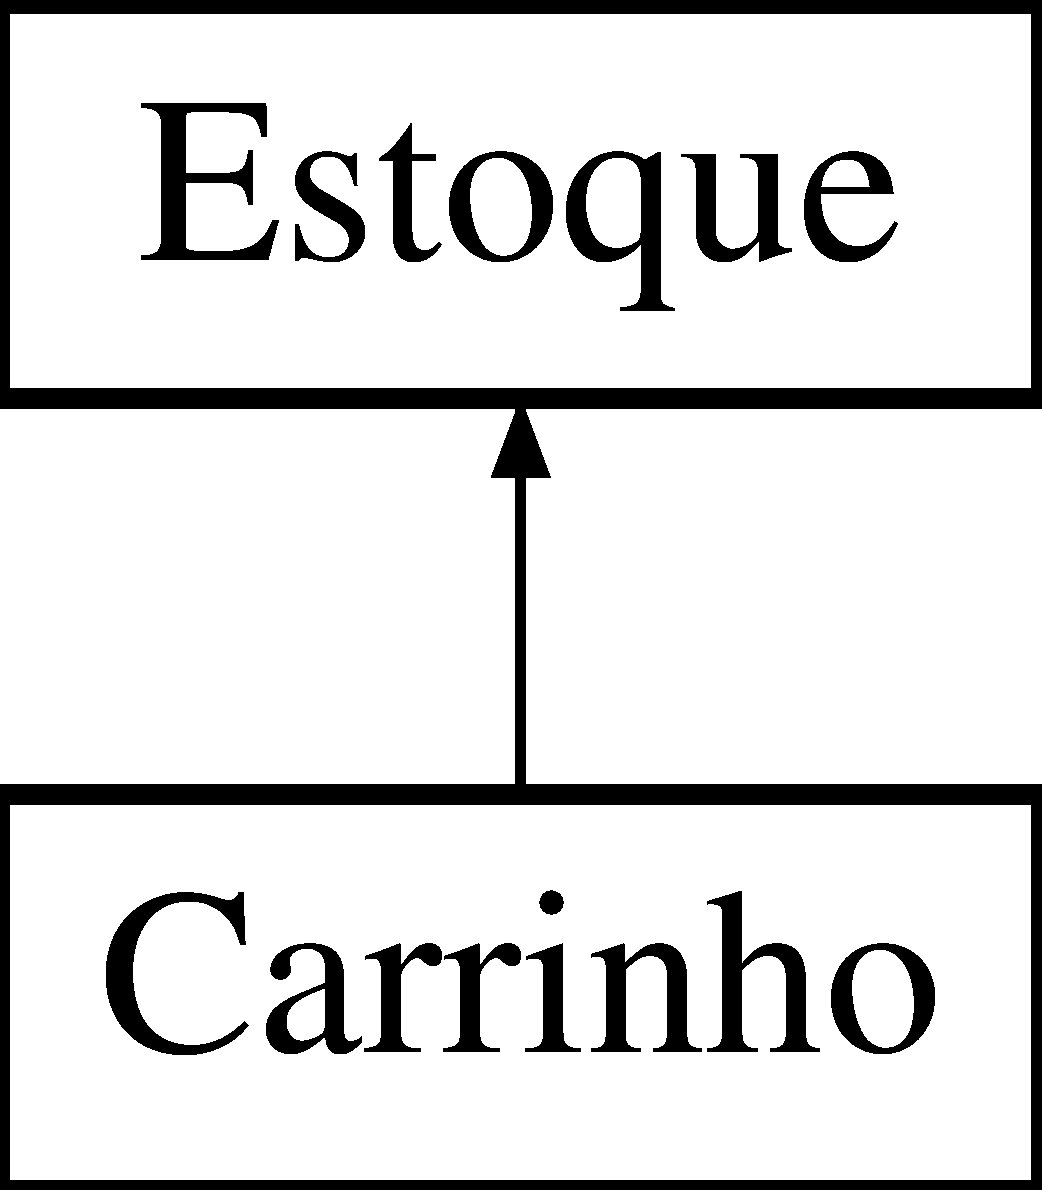
\includegraphics[height=2.000000cm]{class_carrinho}
\end{center}
\end{figure}
\subsection*{Métodos Públicos}
\begin{DoxyCompactItemize}
\item 
\mbox{\Hypertarget{class_carrinho_ab9191572529ba02cfc13366fbc80d7cc}\label{class_carrinho_ab9191572529ba02cfc13366fbc80d7cc}} 
double {\bfseries get\+\_\+valor\+\_\+produtos} ()
\item 
\mbox{\Hypertarget{class_carrinho_a1ffd510925552a0433155a20c98ab3bd}\label{class_carrinho_a1ffd510925552a0433155a20c98ab3bd}} 
double {\bfseries get\+\_\+desconto} ()
\item 
\mbox{\Hypertarget{class_carrinho_ade44d088d0842ca044e3dcf0dcf6f3d3}\label{class_carrinho_ade44d088d0842ca044e3dcf0dcf6f3d3}} 
double {\bfseries get\+\_\+total} ()
\item 
\mbox{\Hypertarget{class_carrinho_aba002453bd5e4bd36f3a25308c1f0d4d}\label{class_carrinho_aba002453bd5e4bd36f3a25308c1f0d4d}} 
void {\bfseries add\+\_\+valor\+\_\+produto} (int valor)
\item 
\mbox{\Hypertarget{class_carrinho_acea5cf443cba7cdf48e9b2019cbd0a28}\label{class_carrinho_acea5cf443cba7cdf48e9b2019cbd0a28}} 
void {\bfseries set\+\_\+desconto} (int desconto)
\item 
\mbox{\Hypertarget{class_carrinho_a1752b97a89f2c22c4cca9d140a74b56b}\label{class_carrinho_a1752b97a89f2c22c4cca9d140a74b56b}} 
void {\bfseries set\+\_\+total} (int total)
\item 
\mbox{\Hypertarget{class_carrinho_aca1d82097c740cae4e0d1d9365cd0abc}\label{class_carrinho_aca1d82097c740cae4e0d1d9365cd0abc}} 
void {\bfseries imprime\+\_\+produtos} (bool socio)
\item 
\mbox{\Hypertarget{class_carrinho_af7bb676480c12ac3d56ecd92a9eab00f}\label{class_carrinho_af7bb676480c12ac3d56ecd92a9eab00f}} 
void {\bfseries atualiza\+\_\+carrinho} (int id, std\+::vector$<$ \hyperlink{class_produto}{Produto} $\ast$$>$ estoque)
\item 
\mbox{\Hypertarget{class_carrinho_a010e07131379a9f1445d889fce3df5e6}\label{class_carrinho_a010e07131379a9f1445d889fce3df5e6}} 
bool {\bfseries possui\+\_\+estoque} ()
\item 
\mbox{\Hypertarget{class_carrinho_a9458dccb325cf853cfa082eb930ae5b7}\label{class_carrinho_a9458dccb325cf853cfa082eb930ae5b7}} 
void {\bfseries cancelar\+\_\+compra} ()
\item 
\mbox{\Hypertarget{class_carrinho_a80238d9f88c542f136b89289f8602aab}\label{class_carrinho_a80238d9f88c542f136b89289f8602aab}} 
void {\bfseries finalizar\+\_\+compra} ()
\end{DoxyCompactItemize}
\subsection*{Outros membros herdados}


A documentação para esta classe foi gerada a partir dos seguintes arquivos\+:\begin{DoxyCompactItemize}
\item 
/home/italo/git/ep1/inc/carrinho.\+hpp\item 
/home/italo/git/ep1/src/carrinho.\+cpp\end{DoxyCompactItemize}

\hypertarget{class_cliente}{}\section{Referência da Classe Cliente}
\label{class_cliente}\index{Cliente@{Cliente}}
\subsection*{Métodos Públicos}
\begin{DoxyCompactItemize}
\item 
\mbox{\Hypertarget{class_cliente_acef88712e8df8e5824416e1cb2f0dc90}\label{class_cliente_acef88712e8df8e5824416e1cb2f0dc90}} 
{\bfseries Cliente} (std\+::string cpf, std\+::string nome, int idade, std\+::string email, bool socio, std\+::map$<$ std\+::string, int $>$ categorias)
\item 
\mbox{\Hypertarget{class_cliente_a34024580fa30f7d4cc353fef7e99bb7e}\label{class_cliente_a34024580fa30f7d4cc353fef7e99bb7e}} 
std\+::string {\bfseries get\+\_\+cpf} ()
\item 
\mbox{\Hypertarget{class_cliente_adc90064373e2284ae082a0c3b992a18e}\label{class_cliente_adc90064373e2284ae082a0c3b992a18e}} 
std\+::string {\bfseries get\+\_\+nome} ()
\item 
\mbox{\Hypertarget{class_cliente_a473bd67382069aaf7ce1ba1a87f62382}\label{class_cliente_a473bd67382069aaf7ce1ba1a87f62382}} 
int {\bfseries get\+\_\+idade} ()
\item 
\mbox{\Hypertarget{class_cliente_a2858b6744b07aee4e180d8b441eb5c51}\label{class_cliente_a2858b6744b07aee4e180d8b441eb5c51}} 
std\+::string {\bfseries get\+\_\+email} ()
\item 
\mbox{\Hypertarget{class_cliente_ac9c0b9492f85d41e4550129412c26bbe}\label{class_cliente_ac9c0b9492f85d41e4550129412c26bbe}} 
bool {\bfseries is\+\_\+socio} ()
\item 
\mbox{\Hypertarget{class_cliente_a59f059460a81ce455585f5ba021f24f6}\label{class_cliente_a59f059460a81ce455585f5ba021f24f6}} 
std\+::map$<$ std\+::string, int $>$ {\bfseries get\+\_\+categorias} ()
\item 
\mbox{\Hypertarget{class_cliente_a666148cd1cc632a13a15420c4da7e2bd}\label{class_cliente_a666148cd1cc632a13a15420c4da7e2bd}} 
void {\bfseries set\+\_\+nome} (std\+::string nome)
\item 
\mbox{\Hypertarget{class_cliente_aa3d5a858d866ba32e70d08b6e4ebab38}\label{class_cliente_aa3d5a858d866ba32e70d08b6e4ebab38}} 
void {\bfseries set\+\_\+cpf} (std\+::string cpf)
\item 
\mbox{\Hypertarget{class_cliente_a9f42acbe77a66b07d3b2d98bb79ee444}\label{class_cliente_a9f42acbe77a66b07d3b2d98bb79ee444}} 
void {\bfseries set\+\_\+idade} (int idade)
\item 
\mbox{\Hypertarget{class_cliente_a7588a428be8edc0263b141049c3d3115}\label{class_cliente_a7588a428be8edc0263b141049c3d3115}} 
void {\bfseries set\+\_\+email} (std\+::string email)
\item 
\mbox{\Hypertarget{class_cliente_aa119e8d42b86f38a9c293f8f7e7aae01}\label{class_cliente_aa119e8d42b86f38a9c293f8f7e7aae01}} 
void {\bfseries set\+\_\+socio} (int socio)
\item 
\mbox{\Hypertarget{class_cliente_a56cd7e779fc5b92fc51d1fe25e340cdf}\label{class_cliente_a56cd7e779fc5b92fc51d1fe25e340cdf}} 
void {\bfseries set\+\_\+categorias} (std\+::map$<$ std\+::string, int $>$ categorias)
\item 
\mbox{\Hypertarget{class_cliente_aa94393f1e6da2e82c89d83d384e0b9e9}\label{class_cliente_aa94393f1e6da2e82c89d83d384e0b9e9}} 
void {\bfseries add\+\_\+categoria} (std\+::string cat, int qnt)
\item 
\mbox{\Hypertarget{class_cliente_a609b2a9404acd81cb19153fa61b5edd0}\label{class_cliente_a609b2a9404acd81cb19153fa61b5edd0}} 
void {\bfseries add\+\_\+categorias} (std\+::vector$<$ \hyperlink{class_produto}{Produto} $\ast$$>$ carrinho)
\item 
\mbox{\Hypertarget{class_cliente_a0e98197e7452264fd968b2600c126a9e}\label{class_cliente_a0e98197e7452264fd968b2600c126a9e}} 
void {\bfseries get\+\_\+recomendacao} (std\+::vector$<$ \hyperlink{class_produto}{Produto} $\ast$$>$ estoque)
\end{DoxyCompactItemize}


A documentação para esta classe foi gerada a partir dos seguintes arquivos\+:\begin{DoxyCompactItemize}
\item 
/home/italo/git/ep1/inc/cliente.\+hpp\item 
/home/italo/git/ep1/src/cliente.\+cpp\end{DoxyCompactItemize}

\hypertarget{class_clientela}{}\section{Referência da Classe Clientela}
\label{class_clientela}\index{Clientela@{Clientela}}
\subsection*{Métodos Públicos}
\begin{DoxyCompactItemize}
\item 
\mbox{\Hypertarget{class_clientela_ac058383888ad0e9902f4ca864b24a7ef}\label{class_clientela_ac058383888ad0e9902f4ca864b24a7ef}} 
std\+::vector$<$ \hyperlink{class_cliente}{Cliente} $\ast$ $>$ {\bfseries get\+\_\+clientes} ()
\item 
\mbox{\Hypertarget{class_clientela_a3fbafd57a0e87cc79355b4aa37e29b81}\label{class_clientela_a3fbafd57a0e87cc79355b4aa37e29b81}} 
\hyperlink{class_cliente}{Cliente} $\ast$ {\bfseries get\+\_\+cliente} (std\+::string cpf)
\item 
\mbox{\Hypertarget{class_clientela_adfa1e93926a2423b2c36010f74a54dca}\label{class_clientela_adfa1e93926a2423b2c36010f74a54dca}} 
void {\bfseries carrega\+\_\+clientes} ()
\item 
\mbox{\Hypertarget{class_clientela_a2f2aae471f8b737a6bad97234d14577b}\label{class_clientela_a2f2aae471f8b737a6bad97234d14577b}} 
bool {\bfseries cliente\+\_\+existe} (std\+::string cpf)
\item 
\mbox{\Hypertarget{class_clientela_a1548d63a41bd54376abb8c6febd37eb7}\label{class_clientela_a1548d63a41bd54376abb8c6febd37eb7}} 
void {\bfseries cadastrar\+\_\+cliente} (std\+::string cpf)
\item 
\mbox{\Hypertarget{class_clientela_ae726bfd284d8db4f25269ef0579cd761}\label{class_clientela_ae726bfd284d8db4f25269ef0579cd761}} 
void {\bfseries add\+\_\+cliente} (\hyperlink{class_cliente}{Cliente} $\ast$pessoa)
\item 
\mbox{\Hypertarget{class_clientela_a290fded8d0f603102d3e2ec530413754}\label{class_clientela_a290fded8d0f603102d3e2ec530413754}} 
void {\bfseries atualiza\+\_\+clientela} ()
\end{DoxyCompactItemize}


A documentação para esta classe foi gerada a partir dos seguintes arquivos\+:\begin{DoxyCompactItemize}
\item 
/home/italo/git/ep1/inc/clientela.\+hpp\item 
/home/italo/git/ep1/src/clientela.\+cpp\end{DoxyCompactItemize}

\hypertarget{class_estoque}{}\section{Referência da Classe Estoque}
\label{class_estoque}\index{Estoque@{Estoque}}
Diagrama de Hierarquia para Estoque\+:\begin{figure}[H]
\begin{center}
\leavevmode
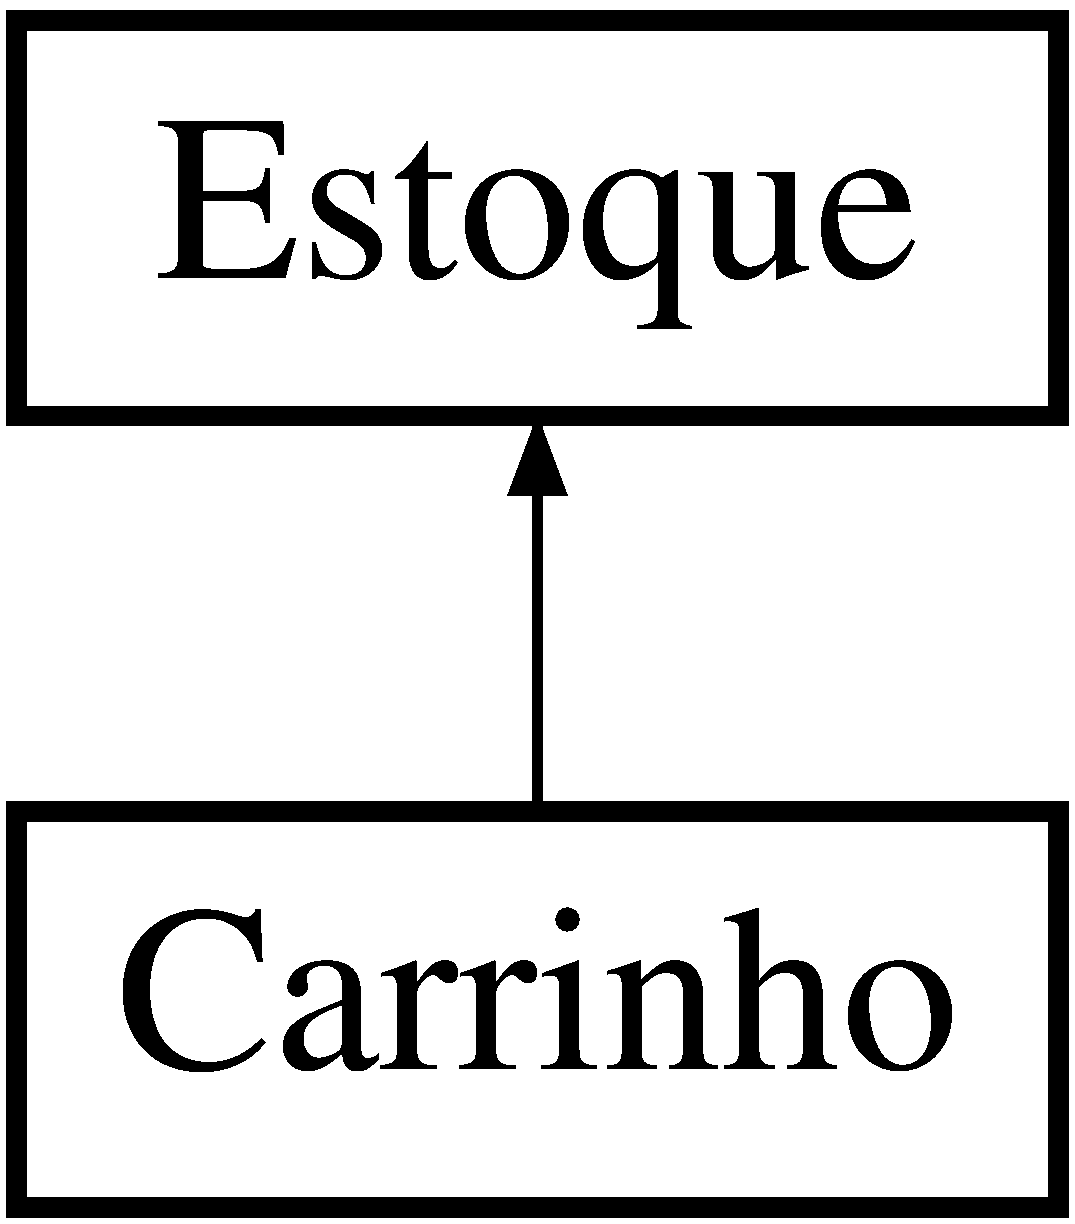
\includegraphics[height=2.000000cm]{class_estoque}
\end{center}
\end{figure}
\subsection*{Métodos Públicos}
\begin{DoxyCompactItemize}
\item 
\mbox{\Hypertarget{class_estoque_a109a5b787075cbba0f4eed2e7ec11a93}\label{class_estoque_a109a5b787075cbba0f4eed2e7ec11a93}} 
std\+::vector$<$ \hyperlink{class_produto}{Produto} $\ast$ $>$ {\bfseries get\+\_\+produtos} ()
\item 
\mbox{\Hypertarget{class_estoque_a22da426fe25845cbb7eb870176cdaf1e}\label{class_estoque_a22da426fe25845cbb7eb870176cdaf1e}} 
\hyperlink{class_produto}{Produto} $\ast$ {\bfseries get\+\_\+produto} (int id)
\item 
\mbox{\Hypertarget{class_estoque_a62209f5dcf7cea9fb6ed477ba2dfe824}\label{class_estoque_a62209f5dcf7cea9fb6ed477ba2dfe824}} 
void {\bfseries carrega\+\_\+produtos} ()
\item 
\mbox{\Hypertarget{class_estoque_ae18931cd4e0d31690d22d132b49b6f95}\label{class_estoque_ae18931cd4e0d31690d22d132b49b6f95}} 
bool {\bfseries produto\+\_\+existe} (int id)
\item 
\mbox{\Hypertarget{class_estoque_aaff596864575f6c19cbec7a5501d2b8e}\label{class_estoque_aaff596864575f6c19cbec7a5501d2b8e}} 
void {\bfseries cadastrar\+\_\+produto} (int id)
\item 
\mbox{\Hypertarget{class_estoque_a8793cb7574f391925d3eaee240ab6ab2}\label{class_estoque_a8793cb7574f391925d3eaee240ab6ab2}} 
void {\bfseries add\+\_\+produto} (\hyperlink{class_produto}{Produto} $\ast$produto)
\item 
\mbox{\Hypertarget{class_estoque_a78d877f97f9aa74ddf73c1430306cc6d}\label{class_estoque_a78d877f97f9aa74ddf73c1430306cc6d}} 
void {\bfseries imprime\+\_\+produtos} (int modo)
\item 
\mbox{\Hypertarget{class_estoque_a72d2e8d79a26cb338c26afccd3e0b8c9}\label{class_estoque_a72d2e8d79a26cb338c26afccd3e0b8c9}} 
void {\bfseries atualiza\+\_\+estoque} ()
\end{DoxyCompactItemize}
\subsection*{Atributos Protegidos}
\begin{DoxyCompactItemize}
\item 
\mbox{\Hypertarget{class_estoque_a2ca8341c75a2c2c0a6750491eea35809}\label{class_estoque_a2ca8341c75a2c2c0a6750491eea35809}} 
std\+::vector$<$ \hyperlink{class_produto}{Produto} $\ast$ $>$ {\bfseries produtos}
\end{DoxyCompactItemize}


A documentação para esta classe foi gerada a partir dos seguintes arquivos\+:\begin{DoxyCompactItemize}
\item 
/home/italo/git/ep1/inc/estoque.\+hpp\item 
/home/italo/git/ep1/src/estoque.\+cpp\end{DoxyCompactItemize}

\hypertarget{class_produto}{}\section{Referência da Classe Produto}
\label{class_produto}\index{Produto@{Produto}}
\subsection*{Métodos Públicos}
\begin{DoxyCompactItemize}
\item 
\mbox{\Hypertarget{class_produto_a2d39bf9da5853de155e921de135a15b6}\label{class_produto_a2d39bf9da5853de155e921de135a15b6}} 
{\bfseries Produto} (int id, std\+::string nome, double preco, int estoque, std\+::vector$<$ std\+::string $>$ categorias)
\item 
\mbox{\Hypertarget{class_produto_afa508e556ea143dd1dda5f18977e8e0c}\label{class_produto_afa508e556ea143dd1dda5f18977e8e0c}} 
int {\bfseries get\+\_\+id} ()
\item 
\mbox{\Hypertarget{class_produto_aa28bbbb0d745f285ac75c3112a4be427}\label{class_produto_aa28bbbb0d745f285ac75c3112a4be427}} 
std\+::string {\bfseries get\+\_\+nome} ()
\item 
\mbox{\Hypertarget{class_produto_ac4a188fc1517266ae7f9dbab1fea783d}\label{class_produto_ac4a188fc1517266ae7f9dbab1fea783d}} 
double {\bfseries get\+\_\+preco} ()
\item 
\mbox{\Hypertarget{class_produto_a7b237e65ddb678cf24810df56487a24b}\label{class_produto_a7b237e65ddb678cf24810df56487a24b}} 
int {\bfseries get\+\_\+estoque} ()
\item 
\mbox{\Hypertarget{class_produto_a7be9c5aa12a4242a13cac4f624a75167}\label{class_produto_a7be9c5aa12a4242a13cac4f624a75167}} 
int {\bfseries get\+\_\+quantidade} ()
\item 
\mbox{\Hypertarget{class_produto_aa13623909f10100d10bccad2a4e5efe8}\label{class_produto_aa13623909f10100d10bccad2a4e5efe8}} 
std\+::vector$<$ std\+::string $>$ {\bfseries get\+\_\+categorias} ()
\item 
\mbox{\Hypertarget{class_produto_aaa9f6841428285a433fc2f1e391dac65}\label{class_produto_aaa9f6841428285a433fc2f1e391dac65}} 
void {\bfseries set\+\_\+id} (int id)
\item 
\mbox{\Hypertarget{class_produto_aab21a57fdd549b4b3df4f8a4343436a1}\label{class_produto_aab21a57fdd549b4b3df4f8a4343436a1}} 
void {\bfseries set\+\_\+nome} (std\+::string nome)
\item 
\mbox{\Hypertarget{class_produto_a865cb11c47226362c576b14b4987d51a}\label{class_produto_a865cb11c47226362c576b14b4987d51a}} 
void {\bfseries set\+\_\+preco} (double preco)
\item 
\mbox{\Hypertarget{class_produto_a597a7fbdfb12ac5dd160c62d315f113b}\label{class_produto_a597a7fbdfb12ac5dd160c62d315f113b}} 
void {\bfseries set\+\_\+estoque} (int estoque)
\item 
\mbox{\Hypertarget{class_produto_a7236d29a461f9d28f1dc402b98a8e4af}\label{class_produto_a7236d29a461f9d28f1dc402b98a8e4af}} 
void {\bfseries set\+\_\+quantidade} (int quantidade)
\item 
\mbox{\Hypertarget{class_produto_a36a43c3b4cffdf436e02c807e038da81}\label{class_produto_a36a43c3b4cffdf436e02c807e038da81}} 
void {\bfseries add\+\_\+quantidade} ()
\item 
\mbox{\Hypertarget{class_produto_a38d3c34151f2794702862c9bcf2b6de5}\label{class_produto_a38d3c34151f2794702862c9bcf2b6de5}} 
void {\bfseries add\+\_\+categoria} (std\+::string categoria)
\end{DoxyCompactItemize}


A documentação para esta classe foi gerada a partir dos seguintes arquivos\+:\begin{DoxyCompactItemize}
\item 
/home/italo/git/ep1/inc/produto.\+hpp\item 
/home/italo/git/ep1/src/produto.\+cpp\end{DoxyCompactItemize}

\hypertarget{class_programa}{}\section{Referência da Classe Programa}
\label{class_programa}\index{Programa@{Programa}}
\subsection*{Métodos Públicos}
\begin{DoxyCompactItemize}
\item 
\mbox{\Hypertarget{class_programa_a96d5ec8d3b1958e2178b3c5e0bf27510}\label{class_programa_a96d5ec8d3b1958e2178b3c5e0bf27510}} 
void {\bfseries menu} ()
\item 
\mbox{\Hypertarget{class_programa_a708b886d24165437c2087477798abd9e}\label{class_programa_a708b886d24165437c2087477798abd9e}} 
void {\bfseries modo\+\_\+venda} (\hyperlink{class_estoque}{Estoque} \&deposito)
\item 
\mbox{\Hypertarget{class_programa_ac07912eab019ffdb72cd717fcdec70fd}\label{class_programa_ac07912eab019ffdb72cd717fcdec70fd}} 
void {\bfseries modo\+\_\+estoque} (\hyperlink{class_estoque}{Estoque} \&deposito)
\item 
\mbox{\Hypertarget{class_programa_ad4de5d75ac95046986bb0844d7fd8058}\label{class_programa_ad4de5d75ac95046986bb0844d7fd8058}} 
void {\bfseries modo\+\_\+recomendacao} (\hyperlink{class_estoque}{Estoque} \&deposito)
\item 
\mbox{\Hypertarget{class_programa_a81a3c64a8b3daf015ae6f956f6eeef25}\label{class_programa_a81a3c64a8b3daf015ae6f956f6eeef25}} 
int {\bfseries getint} (int min, int max)
\end{DoxyCompactItemize}
\subsection*{Atributos Públicos}
\begin{DoxyCompactItemize}
\item 
\mbox{\Hypertarget{class_programa_ab49f082c3dd56de70b50cd8b1acc7bc1}\label{class_programa_ab49f082c3dd56de70b50cd8b1acc7bc1}} 
bool {\bfseries inicio}
\end{DoxyCompactItemize}


A documentação para esta classe foi gerada a partir dos seguintes arquivos\+:\begin{DoxyCompactItemize}
\item 
/home/italo/git/ep1/inc/programa.\+hpp\item 
/home/italo/git/ep1/src/programa.\+cpp\end{DoxyCompactItemize}

%--- End generated contents ---

% Index
\backmatter
\newpage
\phantomsection
\clearemptydoublepage
\addcontentsline{toc}{chapter}{Índice}
\printindex

\end{document}
